
\documentclass[MTech]{iitmdiss}

\usepackage{times}
\usepackage{setspace}
\usepackage{amsmath,amsthm,amssymb,amsfonts}
\usepackage{verbatim}
\usepackage{floatrow}
\usepackage{fullpage}
%\usepackage{txfonts,pxfonts,amsfonts}
\usepackage[usenames,dvipsnames]{xcolor}


\usepackage{xcolor}
\usepackage{caption}
\usepackage{subfig}
\usepackage{graphicx}

\usepackage[square]{natbib}
\usepackage[colorlinks=true,linkcolor=blue]{hyperref}
%\usepackage{hyperref} % hyperlinks for references.
\usepackage[all]{hypcap}
\usepackage{complexity}
\usepackage[named]{algo}
%\usepackage{algpseudocode}

\newtheorem{thm}{Theorem}
\newtheorem{problem}{Problem}
\newtheorem{corr}{Corollary}
\newtheorem{lma}{Lemma}
\newtheorem{case}{Case}
\newtheorem{rmrk}{Remark}
\newtheorem{prp}{Proposition}
\newtheorem{dfn}{Definition}
\newtheorem{qn}{Question}
\newtheorem{att}{Attempt}
\newtheorem{ex}{Example}
\newtheorem{flaw}{Flaw in Attempt}
% Strut macros for skipping spaces above and below text in tables. 
\def\abovestrut#1{\rule[0in]{0in}{#1}\ignorespaces}
\def\belowstrut#1{\rule[-#1]{0in}{#1}\ignorespaces}

\def\abovespace{\abovestrut{0.20in }}
\def\aroundspace{\abovestrut{0.20in}\belowstrut{0.10in}}
\def\belowspace{\belowstrut{0.10in}}
%%%%%%%%%%%%%%%%%%%%%%%%%


\def\thesistitle{Efficient and Exact Range Search of Chemical Fingerprints from a Large Database}
\def\thesisauthor{Abhik Mondal}


\begin{document}
\bibliographystyle{iitm}
%%%%%%%%%%%%%%%%%%%%%%%%%%%%%%%%%%%%%%%%%%%%%%%%%%%%%%%%%%%%%%%%%%%%%% 
% Title page

\title{\thesistitle}

\author{\thesisauthor}

\date{April 2015}
\department{Computer Science and Engineering}

%\nocite{*}
\begin{singlespace}
\maketitle 
\end{singlespace} 

%%%%%%%%%%%%%%%%%%%%%%%%%%%%%%%%%%%%%%%%%%%%%%%%%%%%%%%%%%%%%%%%%%%%%%
% Certificate
\certificate

\vspace*{0.5in}

\noindent This is to certify that the thesis entitled {\bf {\thesistitle}}, 
submitted by {\bf {\thesisauthor}}, to the Indian Institute of Technology, 
Madras, for the award of the degrees of {\bf Bachelor of Technology} \& {\bf Master of Technology}, 
is a bona fide record of the research work carried out by him under my
supervision. The contents of this thesis, in full or in parts, have not been
submitted to any other Institute or University for the award of any degree or
diploma.

\vspace*{1.4in}
\hspace*{-0.25in}
\begin{singlespace}
\noindent {\bf Dr. Sayan Ranu} \\
\noindent Research Guide \\ 
\noindent Assistant Professor \\
\noindent Dept. of Computer Science and Engineering\\
\noindent IIT-Madras, 600 036 \\
\end{singlespace}
\vspace*{0.20in}
\noindent Place: Chennai\\ 
Date:

%%%%%%%%%%%%%%%%%%%%%%%%%%%%%%%%%%%%%%%%%%%%%%%%%%%%%%%%%%%%%%%%%%%%%%
\acknowledgements
%%%%%%%%%%%%%%%%%%%%%%%%%%%%%%%%%%%%%%%%%%%%%%%%%%%%%%%%%%%%%%%%%%%%%%
% Abstract

\begin{abstract}

Chem-informatics is a field dealing with chemistry and information science, with the primary motivation being the use of data mining, information retrieval and machine learning techniques to make predictions and inferences which can later be verified experimentally. Chemical Compounds are frequently represented as feature vectors, where every feature represents the absence, presence or the frequency count of certain important substructures or other chemical properties. These feature vectors are known as "Chemical Fingerprints" . 

Fast database search is vital especially in drug discovery, where the aim is identifying chemical compounds with high similarity to known drugs. In this work, we are concerned with indexing methods of such data sets of chemical compounds to facilitate rapid range search querying on the database. We propose two techniques for the same. There is no loss of accuracy in any of the two methods (in terms of the answer set) when compared to a complete database linear scan .
	
The first technique uses an indexing technique based on the structure of the M-tree. The standard similarity measure used for chemical fingerprints is the Tanimoto Similarity which satisfies triangle inequality. The M-tree structure helps us exploit this fact. The second technique we describe is based on an Inverted Indexing method, which takes advantage of the sparsity and high dimensionality of a typical chemical fingerprint data set. We go on to study the effectiveness of these techniques through various experiments. 

\end{abstract}


\pagebreak

%%%%%%%%%%%%%%%%%%%%%%%%%%%%%%%%%%%%%%%%%%%%%%%%%%%%%%%%%%%%%%%%%
% Table of contents etc.

\begin{singlespace}
\tableofcontents
\thispagestyle{empty}

\listoftables
\addcontentsline{toc}{chapter}{LIST OF TABLES}
\listoffigures
\addcontentsline{toc}{chapter}{LIST OF FIGURES}
\end{singlespace}

\pagebreak


%The main text will follow from this point so set the page numbering
%to arabic from here on.
\pagenumbering{arabic}
%%%%%%%%%%%%%%%%%%%%%%%%%%%%%%%%%%%%%%%%%%%%%%%%%%
% Introduction.
%
%% A category with the (minimum) three required fields
%\category{H.4}{Information Systems Applications}{Miscellaneous}
%%A category including the fourth, optional field follows...
%\category{D.2.8}{Software Engineering}{Metrics}[complexity measures, performance measures]
%
%\terms{Theory}
%
%\keywords{ACM proceedings, \LaTeX, text tagging} % NOT required for Proceedings

\section{Introduction}
Chem-informatics is largely concerned with the task of mining large chemical datasets. Typical applications of this include drug discovery, catalyst analysis and experiment predictions. Usually chemicals are represented as "Chemical Fingerprints".Chemical fingerprints are used for identification of chemicals. They are characteristics or distinctive patterns which help describe them. The comparison of chemical molecules is difficult but if we convert the molecules into bit-strings or into vector format it makes it easier to do a comprehensive comparison. A primary reason for using chemical fingerprints is scalability. We know that sub-graph isomorphism is an NP-complete problem making it difficult to find similarity between two molecules represented in a graphical format. When the data is represented in a vector string, techniques are more scalable in terms of size of query molecules and time to accomplish a similarity detection task.\\

Chemical fingerprints can be built based on structure properties like substructure features. In binary fingerprints each bit represents the presence or absence of specific chemical property like substructure presence. For example the bits could represent the count of individual chemical atoms like carbon, oxygen, hydrogen or the number of saturated or unsaturated aromatic carbon only, nitrogen containing or non-aromatic rings. The reason why substructure presence is is an important feature is because it can be used to reduce or filter out candidate mismatches in the sub-graph isomorphism test process. So given two bit-strings or vectors for binary chemical  fingerprints we can intuitively say that the similarity of the two fingerprints is directly proportional to the number of shared bits. \\

	These fingerprints/feature vectors are designed by domain experts and typical features could include information like number of occurrences of particular substructures, presence of molecules, bonds between the molecules, etc. Generally the dataset is high dimensional and also highly sparse which inherently makes searching and indexing such chemical data sets challenging. \\
	
	For performing query operation on high dimensional data, it is generally observed that all the indexing techniques perform poorly, as compared to linear scan. This is mainly due to the curse of dimensionality . As dimensions increases the data points are scattered further away in space. In some techniques which use pivots to form clusters like the one we will use, it is difficult to form compact groups with a low cluster radius. Since we are unable to form compact representative groups well, more than often a range query requires a search through the entire database of chemical molecules with no chance of pruning occurring.  Hence, in our work we have used "Linear scan" as our base line technique and have come up with  methods to improve our performance. Our experiments will be evaluated against the linear scan technique. The results of the range search will be verified by comparing the range search result set against that obtained by a linear scan approach.\\

	Various scoring schemes like Tversky, Pearson, Dice, and Kulczynski are available for comparing two given fingerprints \cite{willett2006similarity,swamidass2007bounds}.The most widely used and accepted similarity measure for binary fingerprints is the Tanimoto similarity which is equivalent to the Jaccard Similarity index defined as the size of the intersection of the sets divided by the size of union of the sets. Here the similarity measure would correspond to the number of bits which are 1 for both the sets of the fingerprints divided by the number of bits for which atleast one of the fingerprints is 1. In mathematical terms,for binary fingerprints X and Y ,where $X_i$ is the $i^th$ bit of X we define Tanimoto similarity as\[ T_s(X,Y) = \frac{\sum \limits_i X_i \wedge Y_i}
{\sum \limits_i X_i \vee Y_i} \] Here we can show that $1-T_s$ is a proper distance metric preserving triangle inequality which will allow us to use index structures which exploit the property, like M-trees. One challenge which we face here is the extension of the said similarity measure /distance metric to non binary fingerprints. Non binary fingerprints are basically feature vectors where each feature value is a count and not necessary signifying absence or presence using bits \\

	Similarity between chemical molecules plays an important role in various aspects of biology and chemistry like protein ligand docking, biological activity prediction,reaction site modelling and mainly drug discovery. Chemical or molecular similarity  plays a pivotal role in modern techniques used to predict chemical compound properties, designing tailor-made chemicals with a predefined and desirable set of properties and most importantly in managing drug design studies by using large databases containing structures of available chemicals.\\

	The first technique we used is that of M-tree \cite{ciaccia1997indexing} based indexing. In this technique we have proposed a novel pivot selection technique, which results in a efficient search time for range queries. We follow this up by embedding the data in to Euclidean space using Lipschitz embedding. We then perform a detailed analysis of the data, and we show that this analysis naturally leads us to inverted indexing. The large size of the data and the sparsity of the data are the primary challenges which we have addressed in this work.\\


%\input{misc.tex}
%\input{questions.tex}
\chapter{Introduction}

%% A category with the (minimum) three required fields
%\category{H.4}{Information Systems Applications}{Miscellaneous}
%%A category including the fourth, optional field follows...
%\category{D.2.8}{Software Engineering}{Metrics}[complexity measures, performance measures]
%
%\terms{Theory}
%
%\keywords{ACM proceedings, \LaTeX, text tagging} % NOT required for Proceedings

\section{Introduction}
Chem-informatics is largely concerned with the task of mining large chemical datasets. Typical applications of this include drug discovery, catalyst analysis and experiment predictions. Usually chemicals are represented as "Chemical Fingerprints".Chemical fingerprints are used for identification of chemicals. They are characteristics or distinctive patterns which help describe them. The comparison of chemical molecules is difficult but if we convert the molecules into bit-strings or into vector format it makes it easier to do a comprehensive comparison. A primary reason for using chemical fingerprints is scalability. We know that sub-graph isomorphism is an NP-complete problem making it difficult to find similarity between two molecules represented in a graphical format. When the data is represented in a vector string, techniques are more scalable in terms of size of query molecules and time to accomplish a similarity detection task.\\

Chemical fingerprints can be built based on structure properties like substructure features. In binary fingerprints each bit represents the presence or absence of specific chemical property like substructure presence. For example the bits could represent the count of individual chemical atoms like carbon, oxygen, hydrogen or the number of saturated or unsaturated aromatic carbon only, nitrogen containing or non-aromatic rings. The reason why substructure presence is is an important feature is because it can be used to reduce or filter out candidate mismatches in the sub-graph isomorphism test process. So given two bit-strings or vectors for binary chemical  fingerprints we can intuitively say that the similarity of the two fingerprints is directly proportional to the number of shared bits. \\

	These fingerprints/feature vectors are designed by domain experts and typical features could include information like number of occurrences of particular substructures, presence of molecules, bonds between the molecules, etc. Generally the dataset is high dimensional and also highly sparse which inherently makes searching and indexing such chemical data sets challenging. \\
	
	For performing query operation on high dimensional data, it is generally observed that all the indexing techniques perform poorly, as compared to linear scan. This is mainly due to the curse of dimensionality . As dimensions increases the data points are scattered further away in space. In some techniques which use pivots to form clusters like the one we will use, it is difficult to form compact groups with a low cluster radius. Since we are unable to form compact representative groups well, more than often a range query requires a search through the entire database of chemical molecules with no chance of pruning occurring.  Hence, in our work we have used "Linear scan" as our base line technique and have come up with  methods to improve our performance. Our experiments will be evaluated against the linear scan technique. The results of the range search will be verified by comparing the range search result set against that obtained by a linear scan approach.\\

	Various scoring schemes like Tversky, Pearson, Dice, and Kulczynski are available for comparing two given fingerprints \cite{willett2006similarity,swamidass2007bounds}.The most widely used and accepted similarity measure for binary fingerprints is the Tanimoto similarity which is equivalent to the Jaccard Similarity index defined as the size of the intersection of the sets divided by the size of union of the sets. Here the similarity measure would correspond to the number of bits which are 1 for both the sets of the fingerprints divided by the number of bits for which atleast one of the fingerprints is 1. In mathematical terms,for binary fingerprints X and Y ,where $X_i$ is the $i^th$ bit of X we define Tanimoto similarity as\[ T_s(X,Y) = \frac{\sum \limits_i X_i \wedge Y_i}
{\sum \limits_i X_i \vee Y_i} \] Here we can show that $1-T_s$ is a proper distance metric preserving triangle inequality which will allow us to use index structures which exploit the property, like M-trees. One challenge which we face here is the extension of the said similarity measure /distance metric to non binary fingerprints. Non binary fingerprints are basically feature vectors where each feature value is a count and not necessary signifying absence or presence using bits \\

	Similarity between chemical molecules plays an important role in various aspects of biology and chemistry like protein ligand docking, biological activity prediction,reaction site modelling and mainly drug discovery. Chemical or molecular similarity  plays a pivotal role in modern techniques used to predict chemical compound properties, designing tailor-made chemicals with a predefined and desirable set of properties and most importantly in managing drug design studies by using large databases containing structures of available chemicals.\\

	The first technique we used is that of M-tree \cite{ciaccia1997indexing} based indexing. In this technique we have proposed a novel pivot selection technique, which results in a efficient search time for range queries. We follow this up by embedding the data in to Euclidean space using Lipschitz embedding. We then perform a detailed analysis of the data, and we show that this analysis naturally leads us to inverted indexing. The large size of the data and the sparsity of the data are the primary challenges which we have addressed in this work.\\



\chapter{Related Work}

In cheminfomatics the problem of fingerprint searching in a large database is well studied. In \citet*{aung2010indexing} they present a new index-based search method called ChemDex (Chemical fingerprint inDexing) for speeding up the fingerprint database search. They propose a novel chain scoring scheme to calculate the Tanimoto (Jaccard) scores of the fingerprints using an early-termination strategy. The fingerprints are horizontally sorted by the total number of 1's they contain. A vertical sorting or rearrangement then takes place such that most of the 1's get pushed towards the left. After the shuffling vertical splits/slices are created in the database. A two tier index structure is created based on total number of 1's each data point has plus the number of 1's in each split. Since we have vertical slices in the database, when a query compound is given they propose a slice by slice fragment filtering.The bounds are calculated in the first slice and only the compounds which cross the threshold are checked for in the second slice. Since they are laterally traversing the slices and filtering after each slice the number of candidates are decreasing at each step hence reducing the time as compared to when we process the fingerprints in full. They come with a scoring technique such that the partial score at each slice is the upper bound for the final similarity score.\\

This field has also been well motivated in \citet*{swamidass2007bounds}. As mentioned in the paper, fingerprint vectors are used to search large databases of small molecules, currently containing millions of entries, using various similarity measures, such as the Tanimoto or Tversky's measures and their variants. They derive simple bounds on these similarity measures and show how these bounds can be used to considerably reduce the subset of molecules that need to be searched.The paper proposes bounds for both single molecule as well as molecule molecule queries. The queries considered by the paper are based on threshold similarity cut-off with a query compound as well as top-k best set. The paper studied the speed-up achieved in query time against query size , query distribution, length of the chemical fingerprints, threshold cut-off for similarity and the total size of chemical database. They show through experiments that their approach achieves linear speed-ups in order of 1 or more magnitude for the fixed threshold query scenario while for top-k queries, they achieve sub-linear speed-ups in range of $O(D^{0.6})$ where D is size of database.\\

A different approach to the same problem can be seen in \citet*{nasr2010hashing} where to speed-up database searches, they proposed to add to each binary fingerprint a short signature integer vector of length M. For a given fingerprint, the i-component of the signature vector counts the number of 1-bits in the fingerprint that fall on components congruent to i modulo M. Given two signatures, they show how one can rapidly compute a bound on the Jaccard-Tanimoto similarity measure of the two corresponding fingerprints, using the intersection bound. These signatures allow one to significantly prune the search space by discarding molecules associated with unfavourable bounds. \\

In \citet*{napolitano2014adaptive}, the authors proposed an adaptive OR based criterion algorithm which is a technique based on adaptive reference points to fasten the process of querying on a large database of chemical compounds represented as binary fingerprints. They also proposed a unifying view between the
context of reference points and the previously proposed hashing techniques like the Bit Bound technique. They evaluated their algorithm by simulating queries against an excerpt from the ChemDB. They showed how their adaptive method was 2-4 times better than the Bit bound technique.  \\

In \citet*{klein2011ct}, the authors proposed a unique indexing method based on a coupling of tree and cycle features to speed up subgraph queries in graph databases. They created their index using an exhaustive feature enumeration method and used a fingerprint algorithm to store the characteristics of the compound graph. The CT-Index is a useful alternative to existing methodologies. They were able to show the scalability of their technique on large databases. \\

\citet*{nasr2012speeding} propose DivideSkip, an inverted index algorithm for similarity search while in \citet*{thiel2014blocked}, the authors present an optimized inverted index algorithm for the calculation of all pairwise similarities on 2D fingerprints of a given data set. They propose an efficient and effective method for the calculation of Tanimoto similarity on binary fingerprints from a large database of chemical compounds by describing a memory efficient representation of fingerprints.

Many of the aforementioned papers present the evaluations of their algorithms only on binary fingerprints . While some of the methods don't extend to non-binary chemical fingerprints, some of the papers just mention that their procedure works on non-binary fingerprints without showing any evaluation. 

We are looking at exact similarity of chemical compounds and not interested in the approximation of the result set. Hence we do not look into methods like Locally sensitive hashing which maximizes the probability of collision of similar items but does not guarantee it. 


\chapter{Problem Formulation}

\section{Problem Statement}

As the title suggests we are interested in fast indexing and searching of chemical fingerprints. We want to propose new indexing techniques which build on current indexing data structures and which will make searching for chemical compounds in the database faster. Our primary goal is to be able to perform queries on our compound database as fast as possible.
We are looking at accurate searching of similar compounds when given a query compound. The similarity of chemical fingerprints is established using the Min-Max distance which is the generalization of Tanimoto distance for non-binary datasets (explained in the next section). We are dealing with exact similarity match and not approximate similarity . We will be looking at different types of queries, namely the range, point and top-k queries .\\

\begin{problem}{
Range queries are defined as follows , where given a fingerprint, say \textit{f}, and a threshold distance \textbf{$\theta$} we want to obtain the set $S$ of all fingerprints, such that 
\begin{equation}
sim(f,g)~ < ~\theta ~~ \Rightarrow  \textbf{$g\in S$}
\end{equation}

}
\end{problem}
 
%
%Top k search queries would require us to find the top k most similar compounds to the query compound. Given a fingerprint, say \textit{f} and a value \textit{k},we want to find the Set $S$ of size k such that 
%\[ sim(f,g) \geq sim(f,h) ~~\forall g \in S ,~\forall h \notin S \] . We haven't looked at these search queries in the experiments as of yet but plan to explore this area in the future.

Our aim as mentioned earlier is to come up with a novel indexing scheme which would make the aforementioned task faster. For range queries we would want to achieve sub-linear search time speeds.The challenge and novelty in our work comes from the fact that, unlike in  \citet*{swamidass2007bounds} and many other state of the art techniques developed in this domain, we are working on non-binary vector fingerprints. 

The indexing time i.e. the time required to index a compound on average is also a concern for us. For any new compound added to the database we would like to be able to add it easily to the index structure without undergoing any major time-consuming changes. We would like our algorithms to scale on large datasets so we will compare our average range search query times on different sizes of the dataset.

An important thing to note here, which is also described in detail in \autoref{exact} is that we are looking at exact threshold similarity searches and not interested in approximate or probabilistic techniques. In the next section we explain properties of the standard similarity measure used in cheminfomatics to compare chemical fingerprints, the Tanimoto similarity and its extension to non-binary datasets as well as how it can be exploited well to our benefit.  



\section{Similarity measure}

As mentioned in the earlier section the main challenge is the fact that we are dealing with non binary fingerprints which has seen very little work. Many of the papers mentioned in the related work suggest that their technique can be extended to non-binary fingerprints but fail to provide any experimental evaluation nor any details about the similarity measure used. We will be using a generalization of the Tanimoto similarity measure to incorporate non binary feature values. 

The Tanimoto coefficient measure for chemical data is defined as $\frac{x}{x+y+z}$, which is the number of features shared by the two compounds divided by the size of union of the non-zero features in the two compounds together . The variable x is the number of features (or number of 1-bits in a binary fingerprint) present in both the compounds while y and z represent the features present in one while not being present in the other. We can observe that the Tanimoto Similarity has a range from 0 to 1, where high cofficient scores indicates a greater similarity among the compounds than lower coefficient scores. One important thing to note here is that a score of 1 doesn't indicate that the compounds are the same, it just denotes the presence of similar substructures, bonds, molecules,etc in both the compounds i.e. their binary signature or fingerprint is identical. 

For non-binary fingerprints we can extend the same Tanimoto coefficient by using non-zero values as 1 . Another alternative is to use the similarity measure known as Min-Max similarity. Min-Max similarity( $M_s$) between two fingerprints X, Y can be formulated as, where $X_i$ is the $i_{th}$ feature value of X \[ M_s(X,Y) = \frac{\sum \limits_{i} min(X_i, Y_i)}{\sum \limits_{i} max(X_i, Y_i)}\]

If the fingerprints are binary, this similarity measure reduces to the Tanimoto coefficient or similarity. We need to ensure that the corresponding distance measure $M_d=1- M_s$is a metric. We can write the distance measure as: 

\[ M_d(X,Y) = 1- M_s(X,Y) = 1- \frac{\sum \limits_{i} min(X_i, Y_i)}{\sum \limits_{i} max(X_i, Y_i)}\]
\[ M_d(X,Y)= \frac{\sum \limits_{i} |X_i - Y_i|}{\sum \limits_{i} max(X_i, Y_i)}\]

We can easily see that $M_d(X,X)=0$ and that if $M_d(X,Y)=0 $ it implies $X_i = Y_i$ for all i, hence implying X=Y. The triangle inequality has been proved in \citet*{lipkus1999proof}. The triangle inequality bounds helps us in the M-tree index structure where we can use the bounds to prune the entire subtree of fingerprints or alternatively include the whole tree in our dataset.






\chapter{Data}
Before we get to the experiments, we will describe the data in this chapter. To get some more insight in to the behaviour of the indexing techniques that we are applying, we perform further analysis of the dat in the hope of getting some useful explanations. We want to ascertain that a typical fingerprint dataset is high dimensional and highly sparse almost follwing a power law sort of distribution with very few features occuring in almost all the points in the chemical database while majority of the features have a non-zero value in very few points. We want to extract patterns in the data which could be exploited for range search querying and point querying.\\

\section{A Typical Fingerprint Dataset Analysis}
We perform a detailed analysis of the data from  \textbf{Dataset 1} to figure out the kind of indexing technique, which needs to be used to optimize our searching time. The statistics that were extracted from the data are as follows:\\

\begin{table}[ht!]
\centering
\caption{Statistics of Data}
\begin{tabular}{|l|c|}
\hline 
Number of data points & 264016 \\ 
Number of unique features is & 785985 \\ 
Maximum number of features in a data point is & 1903 \\ 
Minimum number of features in a data point is  & 7 \\ 
Average number of features in a data point is & 270.602966 \\ 
Maximum number of data point with a feature is & 259110 \\ 
Minimum number of data point with a feature is & 1 \\ 
Average number of data point with a feature is & 90
 \\ 
Maximum value of a feature  & 1870 \\ 
Minimum value of a feature
 & 1 \\ 
Average value of a feature & 1.142210 \\ 
Maximum number of heavy-hitters  & 144 \\ 
Minimum number of heavy-hitters  & 1 \\ 
 Average number of heavy-hitters  & 44.5 \\ 
\hline 
\end{tabular} 
\end{table}

From this we can observe that the data is highly sparse with only about 271 features, on a average, in a point, as opposed to the 785985 unique features. This high sparsity makes the data set an ideal candidate to perform inverted indexing. In inverted indexing, instead of indexing the data points we would index the features. This leads to a large index structure, but we gain on the speed of point query. \\

\begin{figure}[ht!]	
\centering
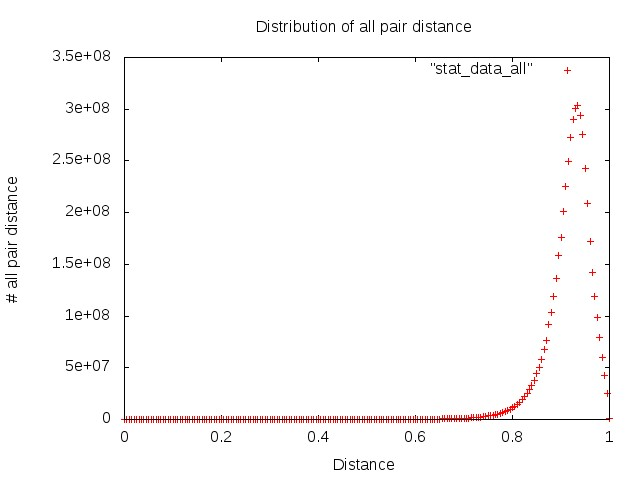
\includegraphics[width=0.7 \columnwidth]{img/all.jpg}
\caption{All pair distances}
\end{figure}
%\pagebreak
\begin{figure}[ht!]	
\centering
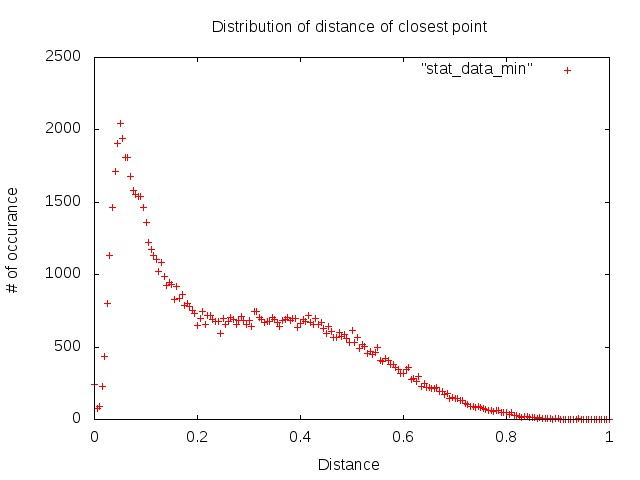
\includegraphics[width=0.7 \columnwidth]{img/min.jpg}
\caption{Distance of the closest point}
\end{figure}

\begin{figure}[ht!]	
\centering
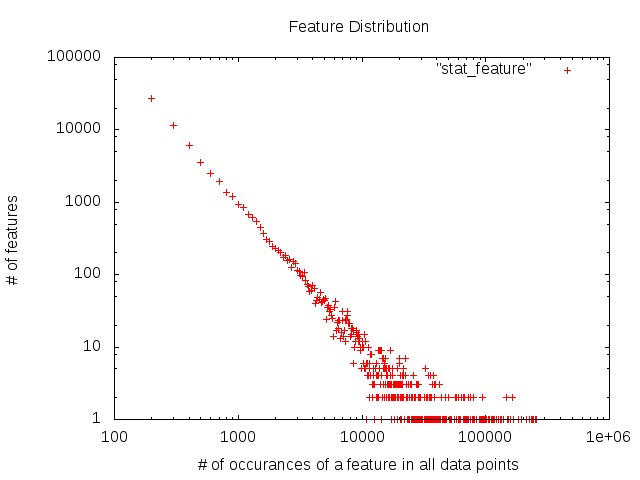
\includegraphics[width=0.7 \columnwidth]{img/feature.jpg}
\caption{Feature distribution}
\end{figure}


\section{Observations on the Data}

What we can observe from the data are the following:
\begin{enumerate}

\item {The being in high dimension, is very much spread out, and hence most of the points are equidistant from each other.}\\

\item {The closest point for most of the points is at distance much greater than 0.4. in fact only 0.007\% of the points have their 1-NN within a distance of 0.4.}\\

\item {the distribution of features among the data points seem to follow a power law distribution (though we have not tried to regress the plot to a function) i.e., even though we have many features only a hand full of them are repeated in most of the points.}\\

\item {One of the most time consuming operations in our algorithms has been the recurring theme of finding the set of maximally separated points, which we called as pivots. It takes hours for the algorithm to converge. Given the distribution of all pairs distance, we cannot hope to improve it further, but we can propose an heuristic streaming algorithm to handle it efficiently.\\ \\
	We can maintain a list of most frequently occurring farthest points. These points are not necessarily the points farthest from each other, but the points which are most frequent in the list farthest points, for each point. This is motivated from the frequency counting problem from streaming as shown in \citet*{metwally2005efficient}.}\\

\item  {We observed that the inverted index we proposed could not be easily generalised  to range queries. This can be further observed from the fact that how skewed the data distribution is.\\ \\
	Given that only 0.007\% of the 1-nn points have distance less that 0.4, we can never achieve a efficient pruning. And in addition the distribution of heavy-hitters (features with occurrence more that 50000) is also very high, We have on an average 44 heavy hitters in a data point. Hence, in the worst case, we will be forced to explore all the points.} \\

\item  {The success of any embedding technique, especially Lipschitz, depends on the ability of the reference set to be representative of the entire data. in our case, given that the entire data is very widely spread, the number of reference set required to well represent the data, becomes very large. This is the reason why Lipschitz did not give the desired results.}
\end{enumerate}


\chapter{Experiments}

In our experiments, we evaluated our indexing techniques on two real world datasets. We have compared our indexing techniques by comparing the running time with that of the state of the art technique  . We are also concerned about the indexing time, especially for the M-tree index structure since we do not want our index procedure to run into hours.

The first dataset is the PubChem(-n and -b) dataset . The second dataset is from DUD, a directory of useful decoys for benchmarking virtual screening. DUD is provided by the Shoichet Laboratory in the Department of Pharmaceutical Chemistry at the University of California, San Francisco (UCSF). DUD is derived from ZINC, a database of commercially avaiilable compounds. To extarct fingerprints we used MOLPRINT2D, a molecular fingerprinting technique.


\section{M-tree based Indexing analysis}	

For these set of experiments the test bed used was a 4 Intel(R) Core(TM) i7-4770 CPU \@ 3.40GHz with 8GB RAM. We have varied several parameters in the experiment and have tried to estimate them emperically. We have used the PubChem-n dataset for all analysis of the M-tree. We use different dataset sizes of 1000, 10,000 and 100,000 number of chemical compounds.

For evaluation purposes we implemented a linear brute force scan to compute the range query and used that as a benchmark for the results. The result set obtained from our technique was compared with the linear brute scan answer set for verification purposes using the fingerprint id's. The query time and the indexing time is averaged over the 500 random query sample data points and the unit in ms per compound. We have varied the following parameters .


\subsection{Limiting Outlier Set Size }

\begin{figure}[ht]	
\centering
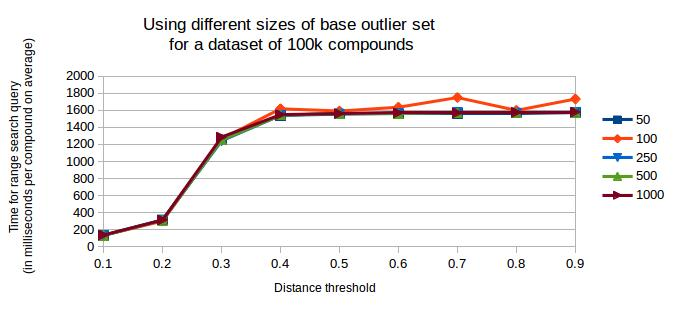
\includegraphics[width=1 \columnwidth]{img/image1.jpg}
\caption{M-tree: Average Range Query time versus Distance Threshold for various sizes of base outlier set}
\label{fig:5.1}
\end{figure}

Just to recap, it is the Minimum limiting size of the outlier set allowed (o). When the outlier set size falls below this limit, we terminate the indexing process.

As seen in \ref{fig:5.1} we can observe that the range search query time is almost constant with change in number of limiting outlier set size. We observed that the outlier base size did not have a significant effect on the query time for range search or on the number of comparisons. The indexing time increases with a lesser outlier base size because the depth of the M-tree increases . The algorithm is applied recursively on the outlier sets, hence when we have a lower base size limit for the outlier sets the number of times the recursion is applied is greater. Since we did not see a great change in query time or number of comparisons we have fixed the size the outlier size limit to 1/100th of the dataset size for all the future experiments.


\begin{figure}[ht!]	
\centering
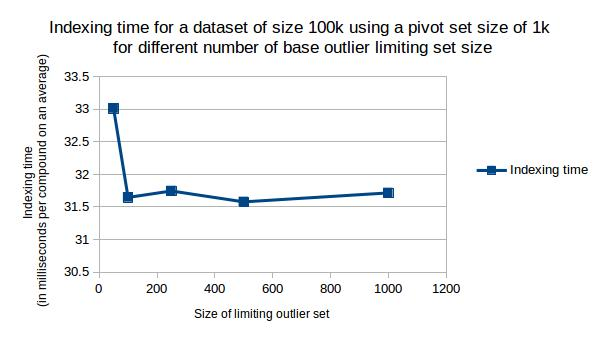
\includegraphics[width=1 \columnwidth]{img/image8.jpg}
\caption{M-tree: Indexing time versus different sizes of base limiting outlier set}
\label{fig:5.2}
\end{figure}


Ideally, indexing time should decrease with increase in number of limiting outlier size. This is because the depth of the M-tree grows with increase in the limitng size of the outlier set. The indexing process is a recursive procedure and termination occurs only when the size of the outlier set falls below the given limiting size. Hence in normal circumstances the indexing time must decrease as we increase the limiting size, but as seen in \autoref{fig:5.2} the decrease is minimal and changing \textit{o} doesn't change the indexing time much. 






\subsection{Pivot Set size}
The pivot set size as described earlier is the number of random pivots chosen at each step of the indexing process (p). \textit{p} determines the number of nodes at every level of the index structure. The number of nodes at each level is equal to p+1.

\autoref{fig:5.3},\autoref{fig:5.4},\autoref{fig:5.5}  show how the range search query time varies versus different distance threshold for different sizes of the pivot set for databases of size 1,000 , 10,000 and 100,000 compounds respectively. We can observe the time is almost similar at high threshold values for different number of pivots. For low theshold values we are succesfully able to prune away all many nodes using triangle inequality. 


\begin{figure}[ht!]	
\centering
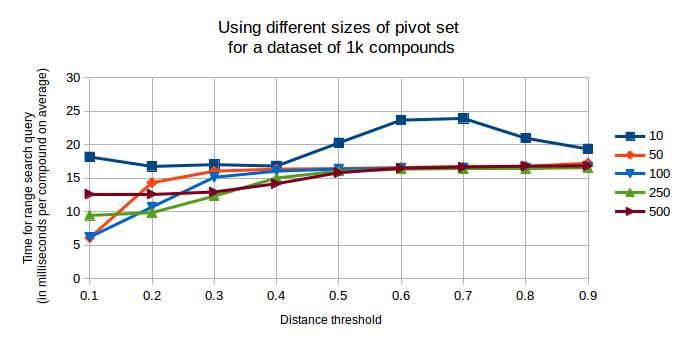
\includegraphics[width=1 \columnwidth]{img/image2.jpg}
\caption{M-tree: Average Range Query time versus Distance Threshold for various sizes of pivot set - 1k database}
\label{fig:5.3}
\end{figure}


\begin{figure}[ht!]	
\centering
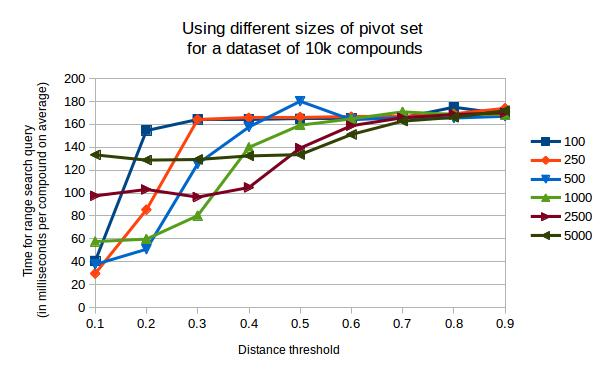
\includegraphics[width=1 \columnwidth]{img/image3.jpg}
\caption{M-tree: Average Range Query time versus Distance Threshold for various sizes of pivot set - 10k database}
\label{fig:5.4}
\end{figure}


\begin{figure}[ht!]	
\centering
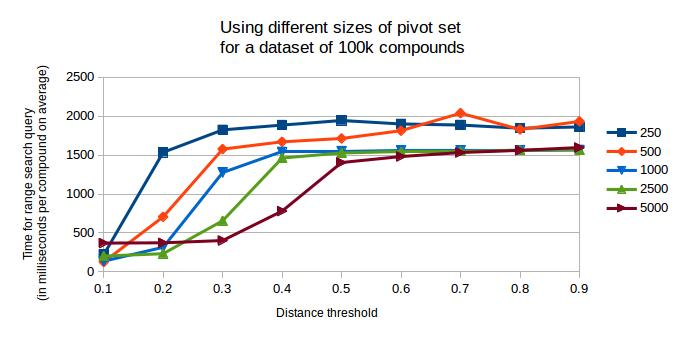
\includegraphics[width=1 \columnwidth]{img/image4.jpg}
\caption{M-tree: Average Range Query time versus Distance Threshold for various sizes of pivot set - 100k database}
\label{fig:5.5}
\end{figure}


We observe that indexing time is increasing almost linearly with increase in the number of pivots chosen at each step of the M-tree algorithm. Even though indexing is an offline process we do not want the indexing time to run into days. If indexing time is very high, updates to the chemical compound database would be very expensive since we need a re-indexing into the chemical database. Hence we need to have a threshold for indexing time.

\begin{figure}[ht!]	
\centering
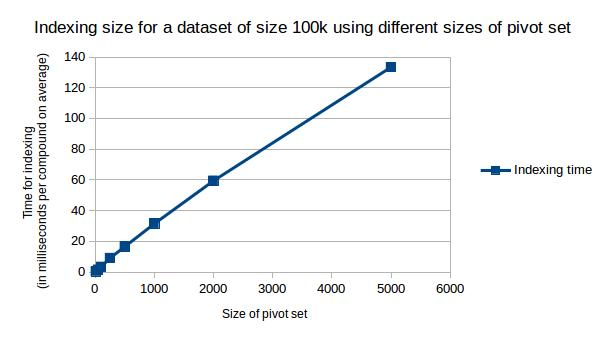
\includegraphics[width=1 \columnwidth]{img/image7.jpg}
\caption{M-tree: Indexing time versus different sizes of pivot set size}
\label{fig:5.6}
\end{figure}



\subsection{Threshold Distance}
As described in earlier sections, the range query distance threshold (t) is thse cutoff used for determining similarity. We observe that range search query time increases monotonically with threshold distance and begins to converge for higher values of threshold distance.  But this seems to hold true only if we use pivots above a particular threshold. 

There are two extremes here. If we use a very high number of pivots most of the time is spent doing computation involving triangle inequality bounds and hence it is not favourable. Similarly if we choose a very low number of pivots, it is not possible to exploit the bounds effectively to decisively prune or include the subtrees from our answer result set. For low number of pivots used we notice that for high and low values of threshold the query time is lower than that for the middle range, where bounds doesn't help well enough.


As seen in \autoref{fig:5.7}, we observe that for low value of threshold at 0.1, the number of pivots to be chosen seems to have a minima between 500 and 1000 for a dataset size of 100k after which it increases . This is because there is a tradeoff between the time saved by pruning the subtrees versus the time utilized in checking if the nodes can be actually pruned.  For a high threshold value of 0.9 it can be seen that we require more number of pivots . 

\begin{figure}[ht!]	
\centering
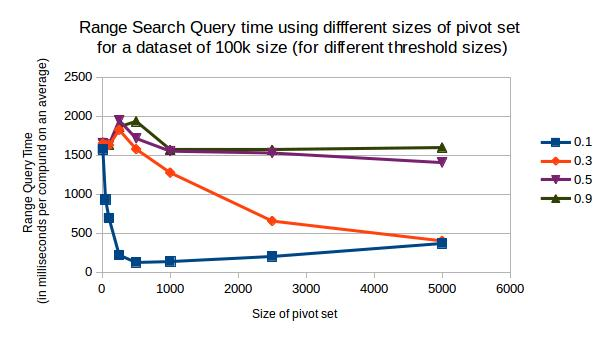
\includegraphics[width=1 \columnwidth]{img/image5.jpg}
\caption{M-tree: Average Range Query time versus various sizes of pivot set for different threshold distances}
\label{fig:5.7}
\end{figure}



\subsection{Dataset Size}
We varied the dataset size for the non-binary version of the PubChem-n to 1000, 10,000 and 100,000 and compared the indexing time as well as range search query time for various thresholds. 


\begin{figure}[ht!]	
\centering
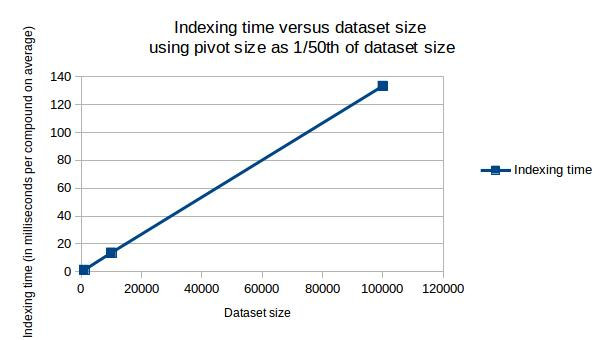
\includegraphics[width=1 \columnwidth]{img/image6.jpg}
\caption{M-tree: Indexing time versus dataset size}
\label{fig:5.8}
\end{figure}

\begin{figure}[ht!]	
\centering
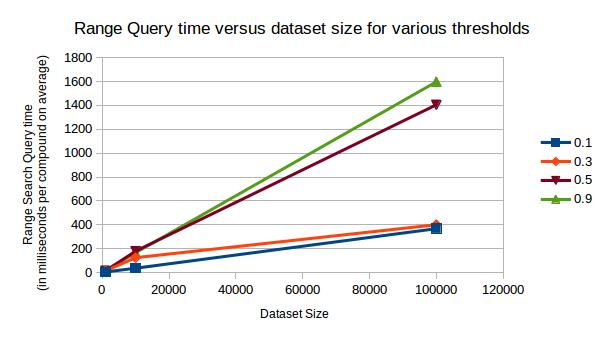
\includegraphics[width=1 \columnwidth]{img/image9.jpg}
\caption{M-tree: Range Query time versus dataset size}
\label{fig:5.9}
\end{figure}


As seen in \autoref{fig:5.9}, we can observe that for a particular value of the distance threshold , the range search query time also increases linearly with dataset size . The slope is higher for higher values of threshold distance.

As seen in \autoref{fig:5.8} we can observe that the average indexing time per compound on average increases linearly with increase in dataset size . This is as a result of our pivoting method with sampling which reduces the computation. If our pivoting step had been an exhaustive search on the database the curve would have not been linear, 





\section{Inverted Indexing Analysis}

For the below experiments the testbed used was a server with 512GB RAM, 24TB disk space, and 2 quad core Xeon processor. We tested the inverted index structure against both binary as well as non-binary versions of the PubChem-n dataset. For evaluation and verification processes, a complete linear database scan was done as with the M-tree case to compare the result sets. One advantage of Inverted indexing procedure over the M-tree index structure is the much lesser time required for the indexing step. 

Indexing time per compound is observed to be almost constant between 1ms to 2ms per compound on average. As observed in \autoref{fig:5I1} the graph is almost straight parallel to the x-axis for both the binary as well as the non-binary dataset. This is in opposition to the M-tree index structure where the indexing time was increasing with increase in the dataset size. 


\begin{figure}[ht]	
\centering
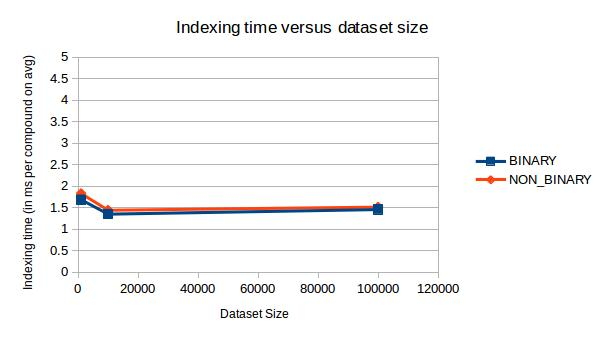
\includegraphics[width=1 \columnwidth]{img/imageI1.jpg}
\caption{Inverted Index: Indexing time versus dataset size for Inverted Indexing}
\label{fig:5I1}
\end{figure}


\autoref{fig:5I2} and \autoref{fig:5I3} show how the range query time graph increases with threshold distances .We can see that in both the figures the time increases monotonically. The double derivative of the curve can be observed to be positive. 

We also observe that the range query time for the binary version of the PubChem-n dataset is lesser compared to the non-binary version of the same dataset. This can be explained by more pruning of features in the binary dataset.

Typically in fingerprint datasets searching is done for a reasonable threshold distance of 0.1 to 0.3 and the search query times uptil 0.3 distance is within a second per compound on average. The figures show that the indexing technique scales well on bigger datasets for low threshold values, better than it scales on higher theshold values.


\begin{figure}[ht]	
\centering
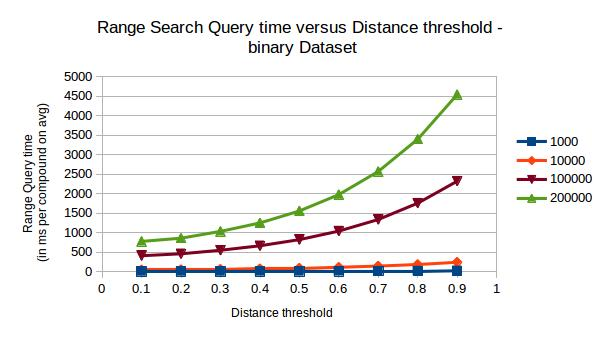
\includegraphics[width=1 \columnwidth]{img/imageI2.jpg}
\caption{Inverted Index: Range Query time versus Distance threshold for different dataset sizes- PubChem-b dataset}
\label{fig:5I2}
\end{figure}

\begin{figure}[ht!]	
\centering
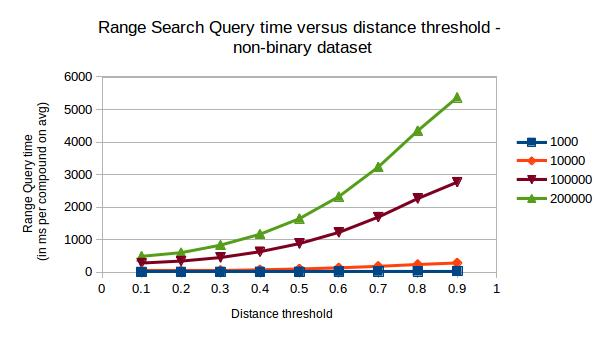
\includegraphics[width=1 \columnwidth]{img/imageI3.jpg}
\caption{Inverted Index: Range Query time versus Distance threshold for different dataset sizes- PubChem-n dataset}
\label{fig:5I3}
\end{figure}


We have also experimented the mentioned improvisations in the Inverted Indexing technique of splitting the heavy hitting features. We observed an increase of about 50-100 ms per compound for the splitting technique.



\section{Comparison of our techniques}

We have compared the three techniques, namely the M-tree indexing technique , the Inverted Indexing technique and the bit bounding technique described in \citet*{swamidass2007bounds}. We have used the PubChem-n, PubChem-b and DUD datasets for our evaluations. A test set of 500 compounds were chosen randomly from the datasets for evaluation purposes. For the experiments, the testbed was a server with 512GB RAM, 24TB disk space, and 2 quad core Xeon processor. 

As observed in \autoref{tab: table1}, comparison of the techniques on the PubChem-b dataset showed for a very low threshold value the M-tree index showed the most promising results, achieving upto two times the speed of the bit bound technique. The inverted index is also able to achieve 2-3 times speedup compared to the bit bound technique. \\



\begin{table}[ht]
\centering
\caption{Comparsion of techniques applied on the PubChem-n fingerprint dataset}
\label{tab: table1}
\begin{tabular}{|c|c|c|c|}
\hline 
Distance threshold & Mtree	& Bit bound	& 	Inverted Indexing \\
\hline
0.1	& 	386.286549	& 820.3638749	&	485.470212\\
0.2	& 	550.1953386	& 1661.947007	&	596.3910451\\
0.3	& 	2473.023198	& 2524.738663	&	826.6685434\\
0.4	& 	4936.808636	& 3363.817437	&	1162.332165\\
0.5	& 	5063.290607	& 4090.751155	&	1643.795028\\
0.6	& 	5122.609976	& 4654.190322	&	2321.426377\\
0.7	& 	5145.041938	& 5018.220471	&	3230.933406\\
0.8	& 	5152.297697	& 5175.073409	&	4346.756728\\
0.9	& 	5178.022697	& 5229.718132	&	5371.661469\\
\hline 
\end{tabular} 
\end{table}

We have shown the effectiveness of out technique on non-binary datasets, a feature unexplored in most papers in the field of research. We can observe from the \autoref{tab: table1} that for high values of distance threshold all three techniques start converging to similar runtime for the range search query. \\

\begin{table}[ht!]
\centering
\caption{Comparsion of techniques applied on the PubChem-b fingerprint dataset}
\label{tab: table2}
\begin{tabular}{|c|c|c|c|}
\hline 
Distance threshold & Mtree	& Bit bound	& 	Inverted Indexing \\
\hline
0.1 & 384.8059272 	&	708.6588827 	&	776.7649653\\
0.2 & 480.429907	  	&  	1444.478385	&	859.3060838\\
0.3 & 1941.113211 	&	2217.534745 	&	1033.699747\\
0.4	& 4896.263139 	&	2995.191962 	&	1251.065067\\
0.5	& 5037.030643 	&	3736.857438 	&	1556.630309\\
0.6	& 5086.700389 	&	4354.433042 	&	1976.196625\\
0.7	& 5118.526736 	&	4859.848535 	&	2568.638003\\
0.8	& 5138.21594	 	& 	5082.24385 	&	3396.452903\\
0.9	& 5168.943088	&	5138.640137 	&	4540.309089\\
\hline 
\end{tabular} 
\end{table}




\begin{table}[ht!]
\centering
\caption{Comparsion of techniques applied on the binary DUD dataset}
\label{tab: table3}
\begin{tabular}{|c|c|c|c|}
\hline 
Distance threshold & Mtree	& Bit bound	& 	Inverted Indexing \\
\hline
0.1 	& 107.1823181	& 146.6163294	& 	29.37458224\\
0.2 & 297.8381414	& 217.9150917	& 	35.10997253	\\
0.3 & 303.2994695	& 272.7101361	& 	39.32821769	\\
0.4 & 295.2179914	& 292.4566623	& 	43.20251988	\\
0.5 & 299.248134 	& 304.6924106	& 	56.92043218	\\
0.6 & 297.995192 	& 294.1471833	& 	69.95566644	\\
0.7 & 289.2738744	& 295.0616706	& 	91.30182238	\\
0.8	& 301.1660971	& 287.0035369	& 	127.5203695	\\
0.9 & 294.3855533	& 289.8519661	& 	191.9871398	\\
\hline 
\end{tabular} 
\end{table}


\autoref{tab: table2} shows the comparison of techniques applied on the PubChem-b dataset while \autoref{tab: table3} shows the comparison of the techniques on the binary DUD dataset. The performance of M-tree index can be seen to be comparable to the bit bound while the performance of the inverted index can be observed to be superior than both the other techniques. For the PubChem-b dataset we observe  that there is always a 2-2.5 times speedup for the inverted index as compared to the bit bound technique. The M-tree index beats the other two techniques for low threshold values but there is a sharp increase in range search query time around 0.3 where the runtime shoots up .


\begin{figure}[ht!]	
\centering
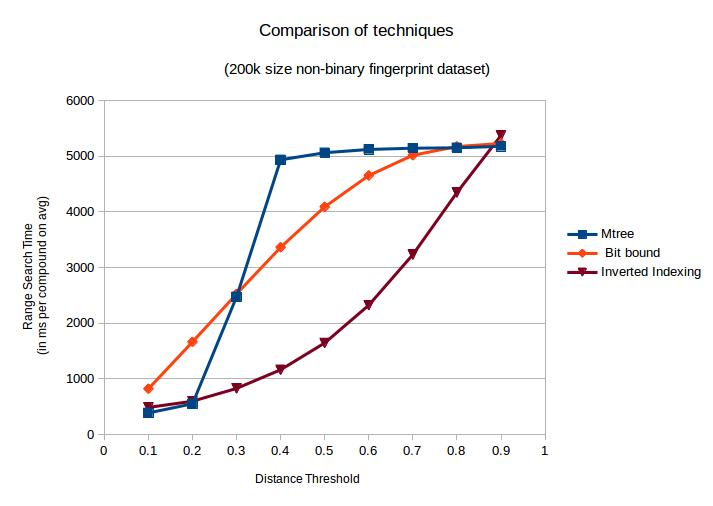
\includegraphics[width=0.75 \columnwidth]{img/imageC1.jpg}
\caption{Comparsion of techniques applied on the PubChem-n fingerprint dataset}
\label{fig:5C1}
\end{figure}


Comparison on the DUD dataset showed that the inverted indexing technique was able to achieve 5-6 times speedup on the M-tree index and the bit bound algorithm. As observed in \autoref{fig:5C1}, \autoref{fig:5C2} and \autoref{fig:5C3} our inverted indexing technique works better than the other two on an average. The M-tree technique works well for lower threshold values, sometimes better than the inverted index technique but fails to scale for higher threshold values. 



\begin{figure}[ht]	
\centering
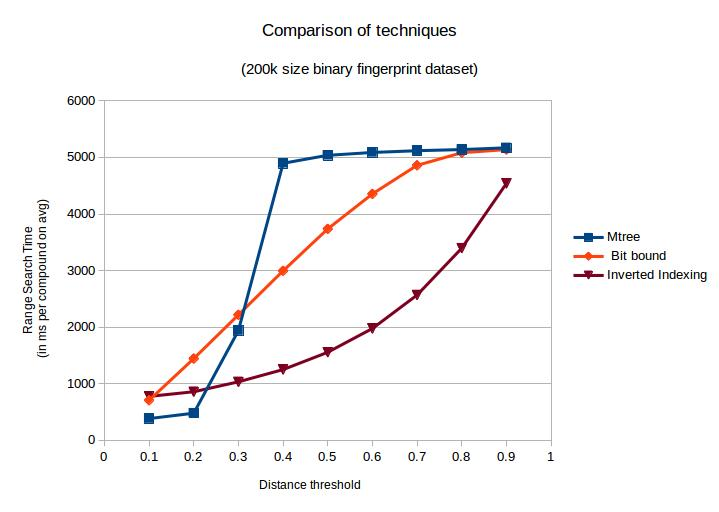
\includegraphics[width=0.75 \columnwidth]{img/imageC2.jpg}
\caption{Comparsion of techniques applied on the PubChem-b fingerprint dataset}
\label{fig:5C2}
\end{figure}

\begin{figure}[ht!]	
\centering
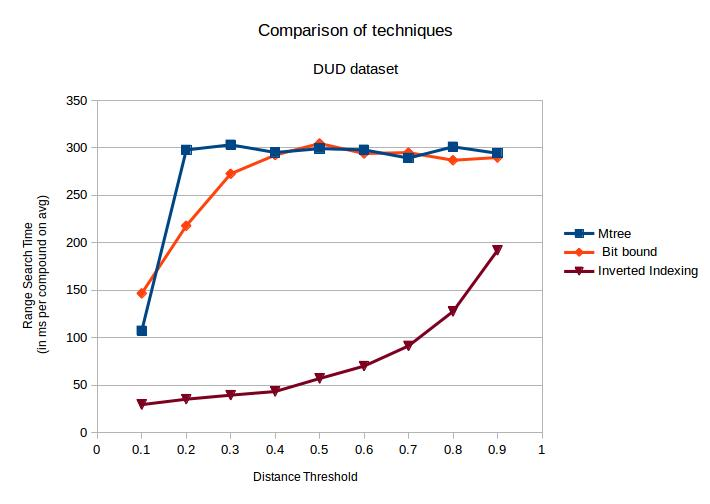
\includegraphics[width=0.75 \columnwidth]{img/imageC3.jpg}
\caption{Comparsion of techniques applied on the binary DUD dataset}
\label{fig:5C3}
\end{figure}

Comparing the M-tree index structure with inverted index technique, we observe the following: The indexing time  per compound on average is constant for the inverted index structure while it varies linearly with size of the dataset for the M-tree. The runtimes for range search queries tends to converge for both the methods as we go towards higher threshold values. The M-tree index shows a sudden increase in runtime for range query at around 0.3 while the curve for the inverted index is smoother. Also, if we were to include a new point into the chemical database the inverted index structure would be simpler since we would just need to update the corresponding feature lists while we would have to undergo a re-indexing for the M-tree index since it would be difficult to add the point randomly into the tree structure.








%
%\chapter{M-tree Based Indexing}
%

M-tree also known as the Metric tree is a tree data structure constructed using a metric distance measure and relies on the triangle inequality for efficient range search queries. Similar to all other tree data structures, an M-tree data structure also has Leaf Nodes and non- Leaf nodes. Every non leaf node has a pointer to its parent node, a pointer to its sub-tree, its object information and a covering radius denoting maximum distance of a node to any node in its sub-tree.Every leaf node keeps a pointer to its parent and object information.\\

The M-tree data structure compartments the objects into nodes, which define regions of the metric space. The maximum capacity of the M-tree is M. For each database object to be indexed, there is an entry $O_j = [ O_j, id(O_j), dist(O_j , P(O_j )) ]$
in some leaf node.  $O_j$ stores the object information, mainly the data point feature values or dimension coordinates, id($O_j$) stores the id of the object and $dist(O_j , P(O_j ))$ stores the distance of it to its parent object. \\

\begin{figure}[ht]	
\centering
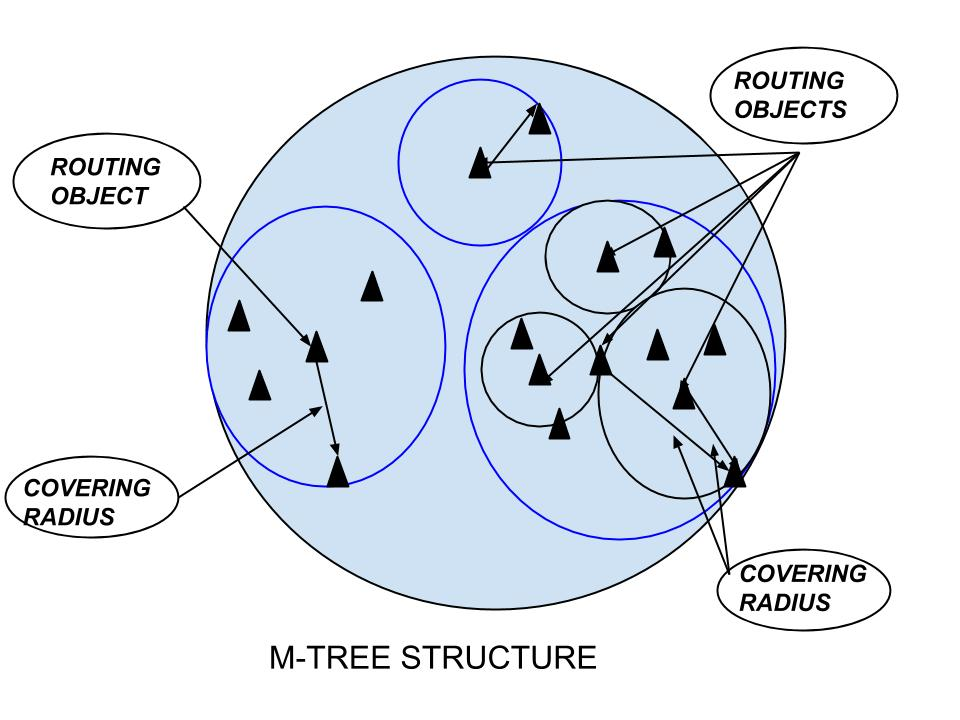
\includegraphics[width=0.7 \columnwidth]{img/mtree.jpg}
\caption{M-tree: Structure overview}
\label{fig:4.0}
\end{figure}

A non-leaf node $O_r$ stores an object information as well as a covering radius $r(O_r)$ and a pointer to a sub-tree i.e. entry $O_r=[ O_r, ptr(T(O_r)), r(O_r), d(O_r, P(O_r)) ]$. One property satisfied is that every object $O_j$ stored in a sub-tree rooted at router object $O_r$ is at at-most $r(O_r)$ distance to it $d(O_j , O_r) ≤ r(O_r)$. M-tree organizes the metric space into a set of, possibly overlapping, regions, to which the same principle is recursively applied.\\




\section{Information in the data structure}

We use a modified data structure similar to the M-tree.We keep the following information in each node of the our modified M-tree: the object identifier of the pivot, i.e fingerprint information of the pivot fingerprint; the pivot also stores a pointer to its children i.e a pointer to a set of fingerprints; a double value which is the distance of the farthest child in its sub-tree and a boolean value which signifies if the pivot is an outlier pivot. We do not require a parent pointer. And the size of each node is determined by the number of pivots chosen at each step of our indexing technique and the base outlier size limit, which are explained later. The following information is stored in each entry of a node in our tree:

\begin{enumerate}
	\item Object identifier $p_i$
	\item Pointer to sub-tree $S_i$
	\item Farthest child i.e. Covering radius $r_i$
	\item Outlier pivot boolean variable
\end{enumerate}

\section{Baseline Indexing approach}
In the baseline approach, we are partitioning the data-set into groups using pivots which enables us to exploit the triangle inequality. The choice of pivots in the baseline approach is done randomly. The number of pivots is determined by two input parameters viz. the number of random pivots chosen at each step and the minimum size of the outlier set allowed at the lowest level. This has been formally explained in the algorithm below. \\

\begin{figure}[ht]	
\centering
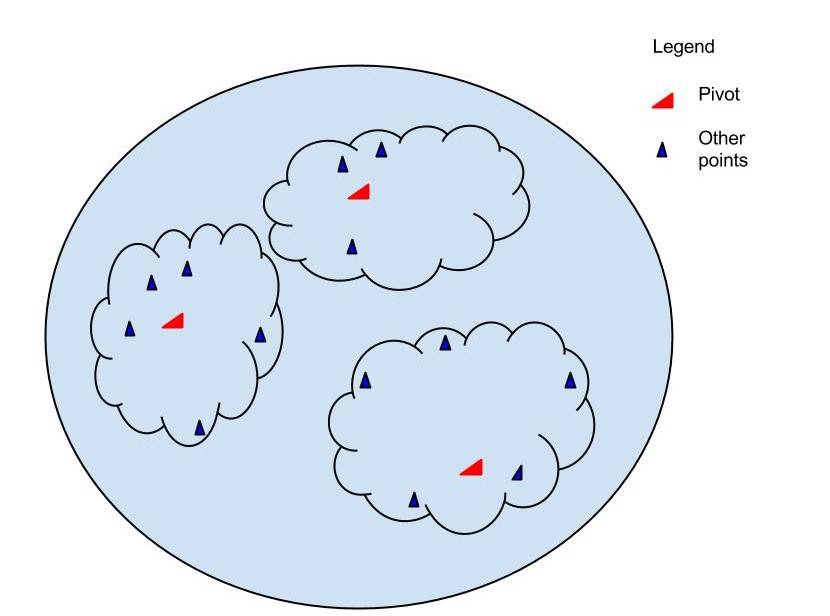
\includegraphics[width=0.7 \columnwidth]{img/image0a.jpg}
\caption{M-tree: Assigning points to a cluster after the pivoting step of the M-tree indexing process}
\label{fig:4.1}
\end{figure}

\begin{figure}[ht]	
\centering
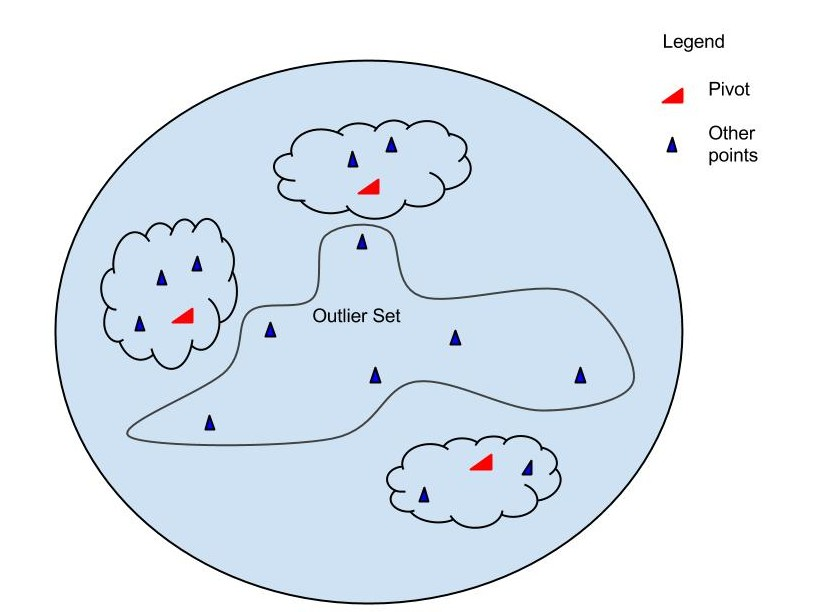
\includegraphics[width=0.7 \columnwidth]{img/image0b.jpg}
\caption{M-tree: Finding the outlier set in the M-tree index structure}
\label{fig:4.2}
\end{figure}
\begin{enumerate}

\item Choose the given number of random pivots from the set. The number of random pivots chosen at this step is a parameter to our experiment and has been varied across different values.

\item After choosing pivots we assign every other chemical compound in the database to one of the pivots based on the similarity to the pivots. A chemical compound is assigned to the pivot which is nearest in distance to it i.e. it has the highest Min-Max similarity with that as compared to other pivots . This is described in \autoref{fig:4.1}.

\item The next step involves ranking all chemical compounds data points by their similarity to their own closest pivot. 

\item We calculate the median similarity among all the chemical compounds in this database and note it as the outlier cut-off/

\item All the chemical compounds with similarity less than the cut-off similarity is called as outliers in this step

\item The outliers are unassigned from the pivots and assigned to the "outlier" pivot. This has been described in \autoref{fig:4.2}

\item We recursively apply this technique on the outlier set until the outlier set size reaches a base limit which is also a parameter to our algorithm.\\

\end{enumerate}


\section{Alternate indexing approach}

We tried an alternate approach where instead of choosing outliers after assigning molecules the most similar pivot we recursively apply the technique on each set. In simpler words, we try to cluster at each step and try to create clusters among each cluster recursively. So in each cluster we choose pivots again and try to assign each of the points to the pivots until we cannot choose more pivots. We can formally explain it as follows.


\begin{enumerate}

\item Choose the given number of random pivots from the set. The number of random pivots chosen at this step is again a parameter to the experiment as previously.

\item The second step is also similar to the earlier indexing technique. After choosing pivots we assign every other chemical compound in the database to one of the pivots based on the similarity to the pivots.
 
\item Instead of choosing outliers now, we work with the same sets and recursively apply this technique on the set until the set size reaches a base limit .

\item The set size limit is set as the number of pivots chosen at each step i.e. the method is applied recursively on the set until the size of the set is lower than the pivot set size making us unable to choose pivots. \\

\end{enumerate}

The previous indexing technique was seen to give us better results. Hence we will be using the earlier technique for all experimental evaluations. One reason we could think of why this technique failed is probably because the tree was becoming more imbalanced and the height was increasing causing querying time to be more.



\section{Choosing pivot}

Instead of randomly choosing pivots at every step we use a Max-Min distance approach where we try to maximize the minimum distance between any two pivot nodes chosen. The procedure can be explained as below:

\begin{enumerate}
	\item Choose a random point.
	\item The second point chosen is such that it is farthest from the first chosen random point. This will require a full database scan
	\item The third point is chosen such that its minimum distance to either of the previous two pivots is maximized.
	\item Iteratively, the $i^{th}$ point is chosen in a fashion such that the minimum of its distance to the previous i-1 points is maximized.
	\item This procedure is repeated till we choose $p$ points where p is the number of pivots to be chosen	\\

\end{enumerate} 

We can observe that this is a very expensive procedure since we are scanning the entire database at every step. We need to compute an all pair similarity initially. At the $i^{th}$ step , the remaining n-i+1 points in  database need to compute its minimum distance to the i-1 points already present in pivot step. Finally choose the point among the n-i+1 points with the maximum distance. This computation is of the O($n^3$).\\
	\begin{equation}
	T(n)=  n^2 + \sum \limits_{i=1}^{n}( (n-i+1)(i-1)  + n-i+1) 
	\end{equation}
	\begin{equation}
	T(n)=O(n^3)
	\end{equation}

We use a sampling technique where we randomly sample a subset of the database and apply the technique described above on the subset. We used a subset size of $\frac{1}{10^{th}}$ the size of the database, approximately about 20,000 points in the subset.


\begin{figure}[ht!]	
\centering
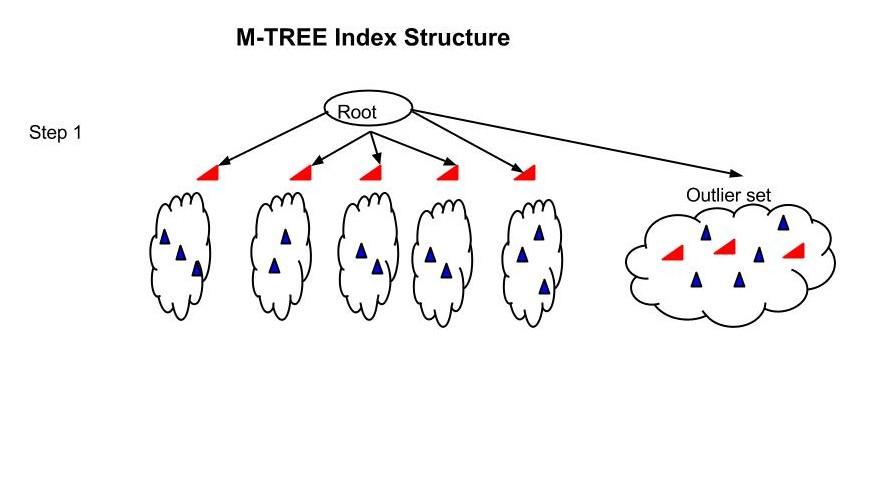
\includegraphics[width=1 \columnwidth]{img/image0d.jpg}
\caption{M-tree: Tree structure Step 1}
\label{fig: step1}
\end{figure}


\begin{figure}[ht!]	
\centering
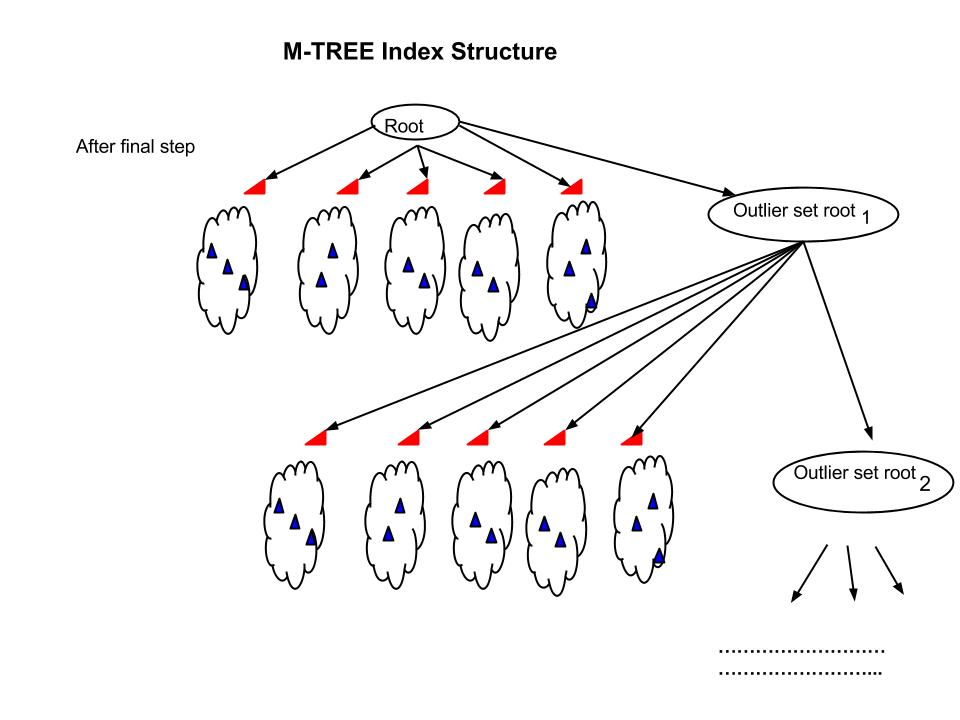
\includegraphics[width=1 \columnwidth]{img/image0e.jpg}
\caption{M-tree: Tree structure - After final step}
\label{fig: final step}
\end{figure}




\section{Range Search Querying}

Given a query chemical fingerprint $q$ and a threshold $\theta $ we want to find the set of chemical fingerprints which satisfy the query. We exploit the triangle inequality for the same. The procedure for range search querying can be described by the following steps\\

\begin{enumerate}
	\item The basic idea is to be able to prune sub-trees based on the covering radius of the pivot of the sub-tree and the distance of the query to the pivot
	 
	\item Let the query fingerprint be q and the fingerprint pivot be $p_i$ of sub-tree $S_i$. We can calculate the maximum distance of any node in $S_i$ from q.We start with the root of the tree as $p_i$
	
	\item Let the covering radius of pivot $p_i$ be $r_i$. Hence the maximum distance of any node in $S_i$ will be $dist(q,p_i)$ + $r_i$. Similarly the minimum distance of any node in $S_i$ is $max(dist(q,p_i)$ - $r_i, 0)$. 
	
	\item Hence we can calculate the range of the distance of any node in $S_i$ to q. 
	
	\item  If the upper bound of the range or the maximum distance is lesser than the threshold distance $\theta$ we can add all the nodes in $S_i$ to our resultant set
	
	\item If the lower bound of the range is greater than the threshold distance $\theta$, we can prune the sub-tree $S_i$ since we can say with certainty that the distance of every node in the sub-tree $S_i$ is greater than  the threshold $\theta$.
	
	\item If there is an intersection in the intervals we recursively apply this technique on the second level of children in the sub-tree $S_i$ until we reach a leaf node.
	
\end{enumerate}



\section{Lipschitz Embedding}

The performance of the M-tree is limited by the fact that the data is very sparse. This results in very loose clusters being formed during the indexing phase. To improve upon this we performed an embedding of the data into Euclidean space using Lipschitz embedding. Lipschitz embedding results in a contractive mapping.\\

Lipschitz embedding is the embedding, or in simpler words, dimensionality reduction of the objects of
a database D with metric distance d onto a k-dimensional feature vector space. The procedure goes as follows:\\
\begin{enumerate}
	\item Choose k subsets of D
	\item Each subset $A_i$ is a reference set
	\item Let the distance of object $p_j$ to set $A_i$ be:\\
	\begin{equation}
	 d(p_j,A_i)= min_{a\epsilon A_{i}} d(p_j,a) 
	\end{equation}

	\item The feature vector f(o) is then defined as:\\
	\begin{equation}
	\label{lip1}
	f(p_j)= {\frac{d(p_j,A_1)}{k},\frac{d(p_j,A_2)}{k}...\frac{d(p_j,A_k)}{k}} 
	\end{equation}

	\item We define the new distance $d'(f(p_j),f(p_k))$ as :\\
	\begin{equation}
	\label{lip2}
	d'(f(p_j),f(p_k)) =\frac{1}{k} \sum \limits_{i=1}^{k} | d(p_j,A_i)-d(p_k,A_i)| 
	\end{equation}

	We notice that the new distance measure is the $L_1$ norm in the new space.
	
	\begin{equation}
	\label{eq:L1}
	L_1(f(p_j),f(p_k)) ~~= \sum \limits_{i=1}^{k} | \frac{d(p_j,A_i)}{k}-\frac{d(p_k,A_i)}{k} | ~~=  \frac{1}{k} \sum \limits_{i=1}^{k} | d(p_j,A_i)-d(p_k,A_i)|  ~~= d'(f(p_j),f(p_k))
	\end{equation}
\end{enumerate}



\begin{figure}[ht!]	
\centering
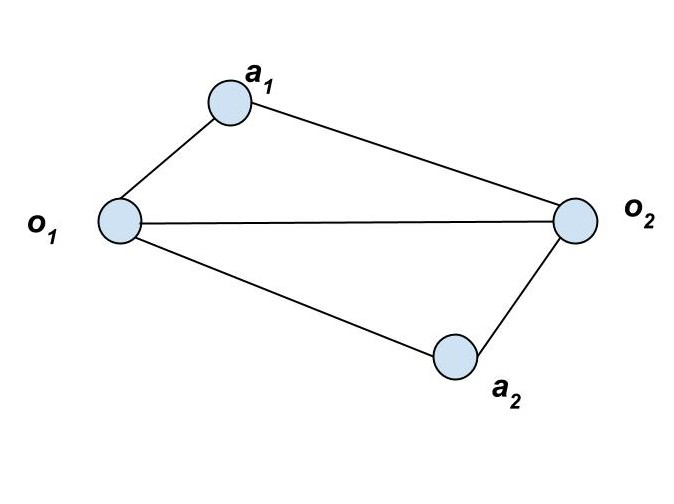
\includegraphics[width=0.4 \columnwidth]{img/lip.jpg}
\caption{Lipschitz: Contractive mapping}
\label{fig: lip}
\end{figure}


\begin{thm}
\label{th0}
A Lipschitz embedding produces a contractive mapping i.e. a Lipschitz embedding of the form $o_i \Rightarrow f(o_i)$ with $f(o_i)$ as defined in \autoref{lip1} and a new distance measure $d'$ as defined in \autoref{lip2} ensures the following:\\

\begin{equation}
	d'(f(o_i),f(o_j)) < d(o_i, o_j)~ \forall ~ i,j
\end{equation} 

\end{thm}

\begin{proof}
	
Consider any arbitrary reference set $A_l$.\\
\begin{equation}
\exists a_1 \in A_l, d(o_1, A_l) = d(o_1, a_1)
\end{equation}
\begin{equation}
\exists a_2 \in A_l, d(o_2, A_l) = d(o_2, a_2)
\end{equation}

as seen in \autoref{fig: lip}.

Now consider $|d(o_1, A_l)-d(o_2, A_l)|$\\

\begin{equation}
\label{der1}
\begin{split}
|d(o_1, A_l)-d(o_2, A_l)| & = |d(o_1, a_1)-d(o_2, a_2)|  \\
 					& = max(d(o_1, a_1)-d(o_2, a_2),d(o_2, a_2)-d(o_1, a_1))\\
 					& \leq  max(d(o_1, a_2)-d(o_2, a_2),d(o_2, a_1)-d(o_1, a_1))\\
 					& \leq d(o_1,o_2)
\end{split}
\end{equation}

Now consider $d'(f(o_i),f(o_j))$ and using \autoref{lip2} and \autoref{der1}\\

\begin{equation}
\label{der2}
\begin{split}
d'(f(o_i),f(o_j)) & = \frac{1}{k} \sum \limits_{l=1}^{k} | d(o_i,A_l)-d(o_j,A_l)| \\
				& \leq \frac{1}{k} \sum \limits_{l=1}^{k} d(o_i,o_j) \\
				& \leq \frac{1}{k} (k d(o_i,o_j)) \\
				& \leq d(o_i,o_j)
\end{split}
\end{equation}

Hence proved that Lipschitz embedding is a contractive mapping.
\end{proof}

\begin{thm}
A Lipschitz embedding of the form $o_i \Rightarrow f(o_i)$ with $f(o_i)$ as defined in \autoref{lip1} and a new distance measure $d'$ as defined in \autoref{lip2} ensures that the new distance measure $d'$ is a metric in the new space.
\end{thm}

\begin{proof}
We have already shown from \autoref{eq:L1} that $d'$ is equivalent to the $L_1$ norm in the new space. Since we know that $L_1$ norm is a metric, it follows the new distance measure $d'$ is also metric in the new space.
\end{proof}

We have chosen the reference sets in our embedding procedure as singleton sets. The choice of these points is done such that they are maximally far apart, i.e., the average and minimum all pairs distance among the reference sets is maximized similar to the method of choosing pivots in our indexing technique. This criteria of selecting the sets was based on the heuristic that farthest point will be maximally representative of the data-set. Since choice of such an optimal set is NP-hard, we perform a randomized set construction.\\

\begin{enumerate}
	\item Choose a random pivot from a sampled set of  data set points

	\item Add the point to our Reference set

	\item Find the point farthest from the reference set from the sampled set of points

	\item Add the point to the reference set

	\item Repeat step 3-4 until Reference set is full\\
\end{enumerate}


Using Lipschitz embedding we propose the following indexing and range search process:
\begin{enumerate}
	\item Embed the data-set using Lipschitz embedding and the pivoting method described above.
	\item Follow the M-tree based indexing process but in this new embedded space.
	\item Carry out the range search to compute the candidate set.  Since from Theorem \autoref{th0}, we know that Lipschitz is contractive we are assured to have our candidate set as a super set of the actual range search result .
	\item We know undergo a similarity computation of all the points in the candidate set to the query in the original space to verify if the candidate point is not a false positive.
\end{enumerate}
Our performance had deteriorated from that of the baseline technique. This is probably because the candidate set which we compute in step 3 is very large and we end up computing similarity for a lot of false positives.

%
%\chapter{Experiments - M-tree Indexing}
%
\section{Experiments - M-tree indexing}

For experiments , the dataset we are using is the size of 200000 chemical compound fingerprints with 500 random query fingerprints chosen from the total set of about 250000 fingerprints. For the experiments the test bed used was a 4 Intel(R) Core(TM) i7-4770 CPU \@ 3.40GHz with 8GB RAM. We have varied several parameters in the experiment .For evaluation purposes we implemented a linear brute force scan to compute the range query and used that as a benchmark for the results. The result set obtained from our technique was also compared with the linear brute scan answer set for verification purposes using the fingerprint id's. The query time and the indexing time is averaged over the 500 query sample data points and the unit in ms per compound. We have varied 3 parameters as described in the subsections below.

\begin{enumerate}

	\item No. of random pivots chosen at each step.

	\item Minimum size of the outlier set allowed (When to stop the indexing)

	\item The range query distance threshold.	\\
\end{enumerate}

\subsection{Different pivots}

We observe that indexing time is increasing almost linearly with the number of pivots chosen at each step. We see that the number of comparisons needed to be made is decreasing with increasing pivots till 2000 for a dataset of about 200000 beyond while indexing time increases significantly We also observe that query time is also similarly reducing with increase in pivots till 2000.

\begin{figure}[ht!]	
\centering
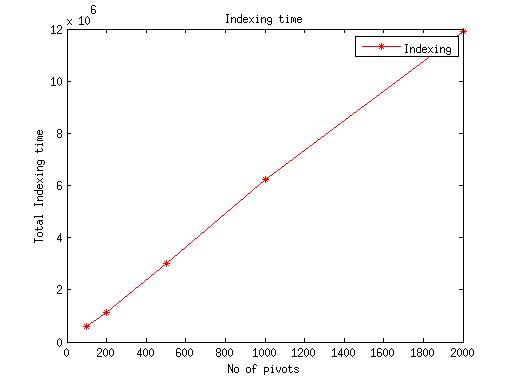
\includegraphics[width=0.35 \columnwidth]{img/indexing_time_n200k_d3_diffpivots.jpg}
\caption{Indexing time (in ms): As seen in the figure indexing time is increasing almost linearly with increase in the number of pivots chosen at each step of the M-tree algorithm. Even though indexing is an offline process we do not want the indexing time to run into days. If indexing time is very high, updates to the chemical compound database would be very expensive since we need a red-indexing into the chemical database. Hence we need to have a threshold for indexing time. The threshold distance used for this experiment was 0.3}
\end{figure}
%\pagebreak

\begin{figure}[ht]	
\centering
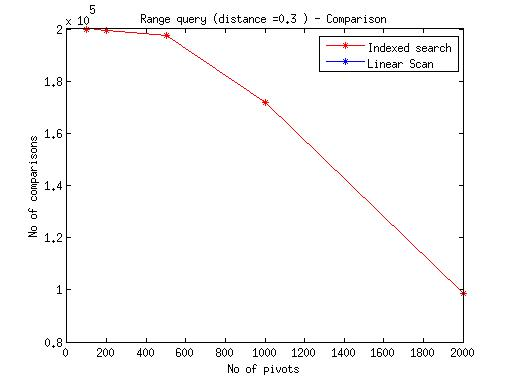
\includegraphics[width=0.35 \columnwidth]{img/comparisons_n200k_d3_diffpivots.jpg}
\caption{Comparisons: As seen in the figure, the number of comparisons i.e. the number of leaves containing chemical compounds which are visited in the M-tree index can be seen to decrease with increase in the number of pivots. We can notice that for number of pivots chosen as 2000, we are able to prune away more than half the nodes in the M-tree . The threshold distance used for this experiment was 0.3}
\end{figure}

\begin{figure}[ht!]	
\centering
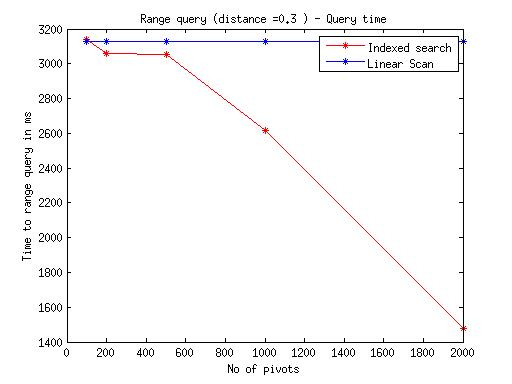
\includegraphics[width=0.35 \columnwidth]{img/query_time_n200k_d3_diffpivots.jpg}
\caption{Query time (in ms): As seen in the figure, the query time can be seen to decrease with increase in the number of pivots. For pivot set size of 2000 we are able to achieve more than 2-times speedup. The linear scan be seen to take about 3100 ms per compound our technique can be seen to take around 1500ms per second for the specific size of 2000 pivots.The threshold distance used for this experiment was 0.3}
\end{figure}


\subsection{Different outlier base size}

We observed that the outlier base size did not have a significant effect on the query time for range search or on number of comparisons. The indexing time increases with a lesser outlier base size because the depth of the M-tree increases . The algorithm is applied recursively on the outlier sets, hence when we have a lower base size limit for the outlier sets the number of times the recursion is applied is greater. Since we did not see a great change in query time or number of comparisons we have fixed the size the outlier size limit to 100 i.e the algorithm terminates when the outlier size becomes lesser than 100.

\subsection{Different distance range queries}

With increasing range distance query , we can see that  both the no of comparisons and query time increases with the distance. This is for a 100,000 data point set. The widely accepted similarity threshold cutoff using the Tanimoto distance is 0.3 which was used in the previous experiments. For lesser distance range queries we get a speed-up of more than 10 times. We have varied the threshold from 0.05 to 0.5 in steps of 0.05. It doesn't make sense to go beyond 0.5 since queries generally want to find similar compounds and 0.5 seems like the maximum threshold. We should expect the curve to fall beyond 0.5. This is because using the triangle inequality bounds, for higher values of threshold distacne we should be able include many subtrees in our answer without having to compare distance of query to all these points. 

\begin{figure}[ht!]	
\centering
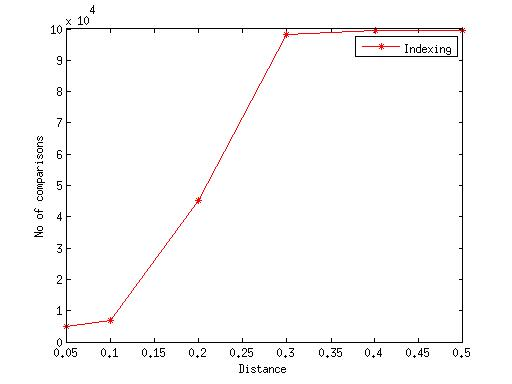
\includegraphics[width=0.35 \columnwidth]{img/comparisons_100k_500p_100o_differentdist.jpg}
\caption{Comparisons: The figure shows the number of comparisons made when different threshold values are used as similarity cutoff. As noticed in the figure, for lower values of threshold , pruning can be applied to more than 90 percent of the nodes . As the threshold reaches 0.5 very little pruning occurs.}
\end{figure}

\begin{figure}[ht!]	
\centering
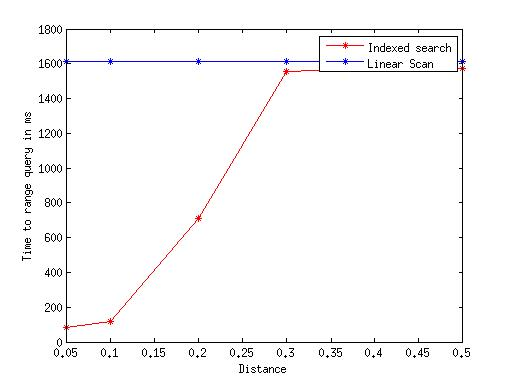
\includegraphics[width=0.35 \columnwidth]{img/query_time_100k_500p_100o_differentdist.jpg}
\caption{Query time (in ms): The figure shows the query time when different threshold values are used as similarity cutoff. As can be seen in the figure, for lower values of threshold almost 15 times speedup can be achieved though for threshold values close to 0.5 the query time increases and becomes comparable to the linear scan query time.}
\end{figure}

%
%\chapter{Inverted Indexing}
%
\section{Inverted indexing}

\subsection{Analysis of the Data}
We performed a detailed analysis of the data to figure out the kind of indexing technique, which needs to be used to optimize our searching time. The statistics that were extracted from the data are as follows:\\

\begin{table}[ht!]
\centering
\caption{Statistics of Data}
\begin{tabular}{|l|c|}
\hline 
Number of data points & 264016 \\ 
Number of unique features is & 785985 \\ 
Maximum number of features in a data point is & 1903 \\ 
Minimum number of features in a data point is  & 7 \\ 
Average number of features in a data point is & 270.602966 \\ 
Maximum number of data point with a feature is & 259110 \\ 
Minimum number of data point with a feature is & 1 \\ 
Average number of data point with a feature is & 90
 \\ 
Maximum value of a feature  & 1870 \\ 
Minimum value of a feature
 & 1 \\ 
Average value of a feature & 1.142210 \\ 
Maximum number of heavy-hitters  & 144 \\ 
Minimum number of heavy-hitters  & 1 \\ 
 Average number of heavy-hitters  & 44.5 \\ 
\hline 
\end{tabular} 
\end{table}

From this we can observe that the data is highly sparse with only about 271 features, on a average, in a point, as opposed to the 785985 unique features. This high sparsity makes the data set an ideal candidate to perform inverted indexing. In inverted indexing, instead of indexing the data points we would index the features. This leads to a large index structure, but we gain on the speed of point query. \\

\subsection{Inverted indexing}

We construct the index structure on features. Our index structure is a chain hashing structure. For a give data point to be inserted in to the structure, for each of it features, we hash the feature and insert the reference to the data point in the chain. In our current implementation we have used a hash table of size 785985, and hence we do not have any collisions. The hash table is maintained as a binary search tree. This structure results in a chain of maximum length 264016.\\

\subsubsection{Point Query}

Point query operation can be very effectively 
implemented in the inverted index structure. To perform this operation we maintain a list of candidate nodes, which needs to be explored sequentially. Our aim is to prune the candidate list as much as possible. This pruning is done by the following observation.\\
Given a point $p$ we look at all its features, and find the list of all nodes associated with the features. It is a straight forward observation that $p$ is present in the dataset only if, it is in the intersection of all the associated point list. This reduces our candidate list to a size, atleast as small as the smallest list, among all the features present in $p$ (which in our case is on an average only 271).\\

\subsubsection{Range Query and K-nn}
Range query and K-nn are much more complicated queries, when compared to a point query. The candidate set in this case is much more diverse and distributed. For example the candidate set for a Range query will be the union of all the point lists associated with the features of $p$, which is the worst case is of the order of $N$. We try to prune this by observing that the minimum number of features in a point is 7, hence we can remove the top 6 features from the index with out affecting the accuracy of searching. But this pruning does not result in any improvement in performance. We shall discuss this further the sections below.\\

%
%\chapter{Experiments - Inverted Indexing}
%\section{Experiments - Inverted Indexing}
The results of point query experiments are as follows\\

\begin{table}[ht!]
\centering
\caption{Point query}
\begin{tabular}{|c|c|c|c|c|}
\hline 
Data size & \multicolumn{2}{c|}{Avg points explored} & \multicolumn{2}{c|}{Avg Time (sec)}\\ 
 & Inverted & linear & Inverted & linear \\ 
\hline 
1000 & 6.87 & 727.6 & 0.02 & 0.764 \\ 
10000 & 54.57 & 7277.67 & 0.1 & 9.76 \\ 
100000 & 334.37 & 73008.21 & 0.5 & 83.09 \\ 
FULL & 1972.75 & 83886.07 & 2.32 & 225.68 \\ 
\hline 
\end{tabular} 
\end{table}

As can be seen our technique is able to achieve up to 100 fold improvement over the linear scan. This was made possible by the pruning that was possible on this dataset. Column 2 and 3 give us a insight into the amount of pruning that was achieved by this technique. We are able to achieve up to 80 times more pruning.

%
%\chapter{Data Characteristics}
%\section{Affect of Data on our Techniques}
To get some more insight in to the behaviour of the indexing techniques that we applied, we performed further more analysis of the data. This gave us some further useful explanations.\\

\begin{figure}[ht!]	
\centering
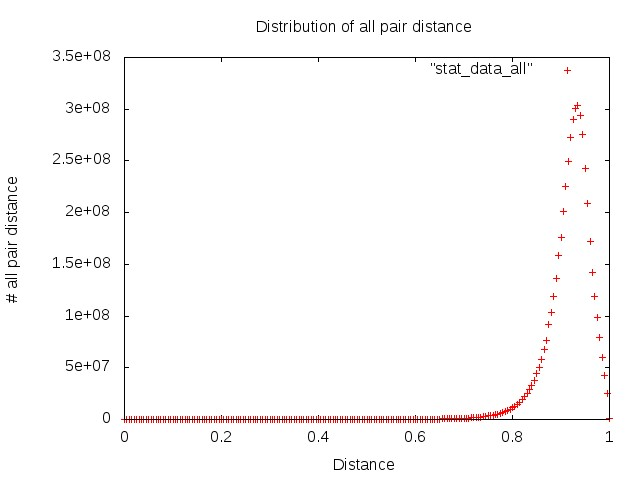
\includegraphics[width=0.35 \columnwidth]{img/all.jpg}
\caption{All pair distances}
\end{figure}
%\pagebreak
\begin{figure}[ht!]	
\centering
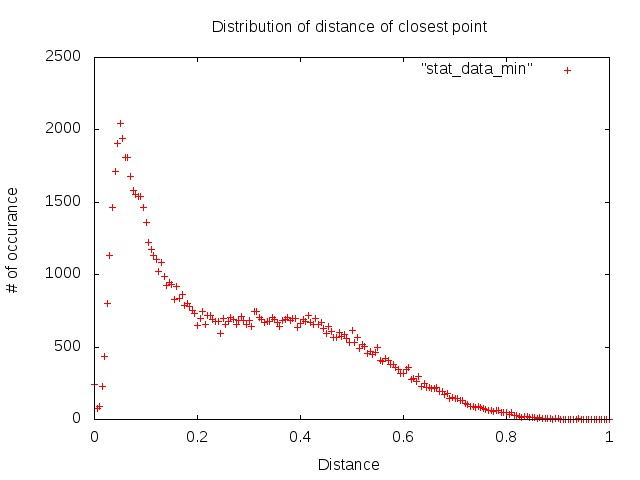
\includegraphics[width=0.35 \columnwidth]{img/min.jpg}
\caption{Distance of the closest point}
\end{figure}

\begin{figure}[ht!]	
\centering
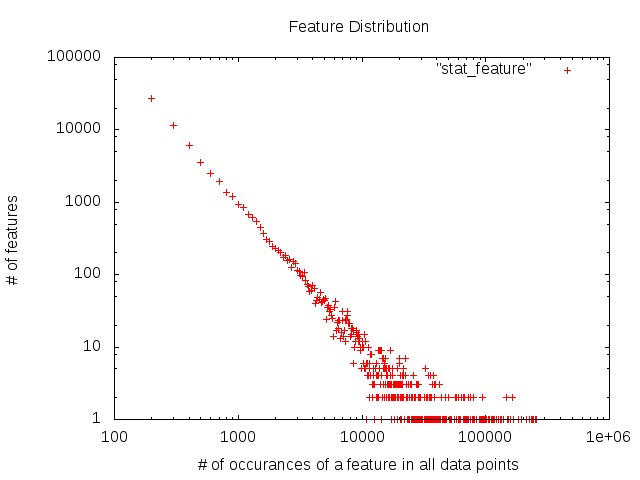
\includegraphics[width=0.35 \columnwidth]{img/feature.jpg}
\caption{Feature distribution}
\end{figure}

What we can observe from the data are the following:
\begin{enumerate}

\item {The being in high dimension, is very much spread out, and hence most of the points are equidistant from each other.}\\

\item {The closest point for most of the points is at distance much greater than 0.4. in fact only 0.007\% of the points have their 1-NN within a distance of 0.4.}\\

\item {the distribution of features among the data points seem to follow a power law distribution (though we have not tried to regress the plot to a function) i.e., even though we have many features only a hand full of them are repeated in most of the points.}\\

\end{enumerate}

These observations have many profound impact on our algorithms.
\begin{enumerate}

\item[A.] {One of the most time consuming operations in our algorithms has been the recurring theme of finding the set of maximally separated points, which we called as pivots. It takes hours for the algorithm to converge. Given the distribution of all pairs distance, we cannot hope to improve it further, but we can propose an heuristic streaming algorithm to handle it efficiently.\\ 
	We can maintain a list of most frequently occurring farthest points. These points are not necessarily the points farthest from each other, but the points which are most frequent in the list farthest points, for each point. This is motivated from the frequency counting problem from streaming as shown in \citet*{metwally2005efficient}.}\\

\item[B.] {We observed that the inverted index we proposed could not be easily generalised  to range queries. This can be further observed from the fact that how skewed the data distribution is.\\ 
	Given that only 0.007\% of the 1-nn points have distance less that 0.4, we can never achieve a efficient pruning. And in addition the distribution of heavy-hitters (features with occurrence more that 50000) is also very high, We have on an average 44 heavy hitters in a data point. Hence, in the worst case, we will be forced to explore all the points.} \\

\item[C.] {The success of any embedding technique, especially Lipschitz, depends on the ability of the reference set to be representative of the entire data. in our case, given that the entire data is very widely spread, the number of reference set required to well represent the data, becomes very large. This is the reason why Lipschitz did not give the desired results.}
\end{enumerate}

%
%\chapter{Conclusion}
%
\section{Conclusions and Future Directions}

In this work we were able to show the effectiveness of M-tree based approach on non-binary feature vectors. Though we could achieve up to 2-fold improvement in query time, we would want to improve this further by doing further analysis.We also were able to effectively exploit the sparsity in data to construct the inverted index, which had given up to 100-fold improvement in query time.The current work has opened up many more avenues for us to explore. We shall be looking into the following areas:\\
\begin{enumerate}
\item Use of streaming algorithm as mentioned in the previous section. 
\item We also observe that we can replace Binary Search Tree in the inverted index technique by a height balanced data structure to result in even more efficient index structure. 
\item One other direction which is a worthy endeavour is the exploitation of the fact that the maximum value taken by any feature is bounded. We may be able to come up with some good bounds on the distance metric based on this, these bound can be in turn used to provide good pruning.  
\item We will also be looking into other dimensionality reduction techniques like principal component analysis, fast map, etc. Since we are looking into exact range search queries, we must be able to give guarantees on the new mapping, preferably a contractive mapping which will be a challenge \\
\end{enumerate}
 
%
%
%\chapter{Future Work}



%%%%%%%%%%%%%%%%%%%%%%%%%%%%%%%%%%%%%%%%%%%%%%%%%%%%%%%%%%%%
% Appendices.
%\appendix
%\chapter{Appendix}
%\input{appendix.tex}
% Bibliography.
\pagebreak
\begin{singlespace}
  \begin{small}
	\bibliography{bibliography}
  \end{small}
\end{singlespace}

%%%%%%%%%%%%%%%%%%%%%%%%%%%%%%%%%%%%%%%%%%%%%%%%%%%%%%%%%%%%

\end{document}
